\documentclass[
  11pt, % 10pt - 12pt
  %letterpaper
  %indonesian
]{assignment}

% Template-specific packages
\usepackage{mathpazo} % Use the Palatino font

\usepackage{graphicx} % Required for including images
\usepackage{booktabs} % Required for better horizontal rules in tables

\usepackage{amsmath} % Math!
\usepackage{listings} % Required for insertion of code
\usepackage{enumerate} % To modify the enumerate environment

% https://castel.dev/post/lecture-notes-2/#including-inkscape-figures-in-a-latex-document
\usepackage{import}
\usepackage{xifthen}
\usepackage{pdfpages}
\usepackage{transparent}
\usepackage{float}

\newcommand{\incfig}[1]{%
    \def\svgwidth{\columnwidth}
    \import{./graphics/}{#1.pdf_tex}
}


\newcommand{\ipAddress}[1]{{\fontfamily{cmtt}\selectfont #1}} % IP Address custom style!

% ! CUSTOM - LST Preset
\lstset{
    language=SQL,
    frame=single, % Frames
    showstringspaces=false, % Don't put marks in string spaces
    numbers=left, % Line numbers on left
    numberstyle=\tiny, % Line numbers styling
    breaklines,
    basicstyle=\fontfamily{cmtt}\selectfont\small,
    columns=fullflexible,
}


%----------------------------------------------------------------------------------------
%	ASSIGNMENT INFORMATION
%----------------------------------------------------------------------------------------

% Student name
\author{Christopher Angelo - 2440041503}
% Institute or school name
\institute{BINUS University\\ Global Class}


% Due date
\date{Nov 25th, 2022}
% Assignment title
\title{Mid Exam Answer}

% Course details
\class{Cloud Technology Practice (CPEN6232010)}
\professor{Mr.\ Santoso Budijono}

%----------------------------------------------------------------------------------------

\begin{document}
\maketitle

%----------------------------------------------------------------------------------------
%	ASSIGNMENT CONTENT
%----------------------------------------------------------------------------------------

\section*{Learning Objective 1}

\begin{problem}
Explain the 3 types of cloud computing models, each with an example!
\end{problem}

\subsection*{LO1: Answer 1}

The three types of cloud computing models are as follow:

\subsubsection*{IaaS} Also known as Infrastructure as a Service, these service providers offer the basic building blocks of cloud computing such as virtual machines, storage, and networking. In this model, the user is completely responsible for the operating system and their respective applications.

Examples of IaaS providers are Amazon Web Services (AWS), Microsoft Azure, and Google Cloud Platform.

\subsubsection*{PaaS} Also known as Platform as a Service, these service providers offer users a platform for developing, running, and managing their applications. In this model, the user is responsible for the application and the data, but the service provider is responsible for the operating system. Usually, developers only need to provide an executable code to run (e.g\@. a Docker container, a shaded JAR file, etc.).

Example of PaaS providers are Heroku, Render.com, Vercel, Google App Engine, and Microsoft Azure App Service.

\subsubsection*{SaaS} Also known as Software as a Service, these service providers offer users a complete software solution. In this model, the user is not responsible for the application, the data, or the operating system. The service provider is responsible for all of these. Usually, the fees that are charges are ongoing operational fees (e.g\@. monthly subscription fees).

Examples of SaaS providers are Zoho, Salesforce Google Workspace, Microsoft Office 365, and Dropbox.

\begin{problem}
Explain in detail the advantages of cloud computing!
\end{problem}

\subsection*{LO1: Answer 2}

Before the existence of Cloud Computing, companies have to buy and maintain their own servers and services. Extra resources such as space and human workforce are needed to uphold these hardware. Starting out initially, there will be a bigger initial expense to acquire. One will also need to consider the resources' capacity; whether it can handle peaks of peaks and not waste any resources when serving over the lowest of depth in processing power. It is very clear that this is a very expensive and time-consuming process which may not be feasible for all company who wants to deploy a modern system.

Cloud Computing solves this problem by providing a platform for companies to rent servers and other computing resources. Instead of spending and investing extra resources on these kind of resources in-situ, you are essentially `offloading' the responsibility to another company who has datacenters worth of servers already setup. Once set up properly, with a pay-as-you-go / subscription pricing model, any spikes or dips in usage may be a time save and a cost saving opportunity. These advantages adds up cumulatively, allowing you to focus on your core business instead of maintaining your own servers on-prem.

\begin{problem}
In implementing cloud computing, the term TCO (Total Cost of Ownership) is known, explain the meaning of the Total Cost of Ownership!
\end{problem}

\subsection*{LO1: Answer 3}

TCO is the total cost of ownership of a product or service. It is the sum estimate of all costs that are incurred during the entire life cycle of a product or service (in this case, a direct and indirect const of running servers). This includes the initial cost, the cost of maintenance, and the cost of disposal where to put is simply:

\[TCO = \text{Initial Cost} + ( \text{Monthly Maintenance Cost} \times \text{Month of Upkeep} ) + \text{Disposal Cost}\]

\begin{problem}
Explain the tools that AWS users can use in implementing the above TCO\@!
\end{problem}

\subsection*{LO1: Answer 4}

AWS provides a tool called AWS Simple Monthly Calculator (and for a more advanced user, AWS Cost Explorer) which allows users to estimate, monitor and visualize their costs `renting' a server from AWS\@. This tool allows users to see their costs in a graphical manner, allowing them to see their costs in a more intuitive way. This tool also allows users to see their costs in a more detailed manner, allowing them to see their costs in a more granular way, identifying pottential cost saving measures in the process.

\section*{Learning Objective 2 - To be verified}

\begin{problem}
What is an AWS Region in AWS Infrastructure, please provide an explanation/example regarding the Region!
\end{problem}

\subsection*{LO2: Answer 1}

An AWS Region is a geographical area that consists of two or more Availability Zones. Each AWS Region is completely isolated from other AWS Regions and most-likely to be far away geographically from each other. This means that data stored in one AWS Region by default cannot be accessed directly by another AWS Region. This is done to ensure that data is stored in a secure manner. If required, access to data in one AWS Region can be granted by using AWS Direct Connect or AWS Virtual Private Network which will be routed through AWS' backbone network.

\begin{problem}
What are Availability Zones (AZs) in AWS Infrastructure, please provide an explanation/example of AZs!
\end{problem}

\subsection*{LO2: Answer 2}

An Availability Zone (AZ) is a data center that is located within an AWS Region. Each AZ is completely isolated from other AZs. This means that data stored in one by default AZ cannot be accessed by another AZ\@. This is done to ensure that data is stored in a secure manner. Though, AWS recommends to replicate data across AZ for redundancy, resiliency and backup purposes. In addition If wanted, user may connect AZ to AZ via a local private link, or AZ to another region via a AWS' backbone network.

\begin{problem}
Explain the relationship between AWS Regions and AZs!
\end{problem}

\subsection*{LO2: Answer 3}

Reiterating on previous answers, every AWS Region has two or more AZs. A region is a physical location within the world where Amazon `clusters' data center. An AZ is simply the said data center which have its own redundancy and resiliency measures. Almost every AWS service is available in every AZ, in fact, you might need to define in which AZ that the service will run.

\begin{problem}
When making our Cloud system have high availability capability, reducing the possibility of data loss, how do we manage those Regions and AZs?
\end{problem}

\subsection*{LO2: Answer 4}

Using AWS, we need to consider the following:

\begin{enumerate}
	\item \textbf{Redundancy} --- Consider having multiple copies of data and / or services in different AZs (or even Region).
	\item \textbf{Latency} --- Consider serving services in the region where it's closest to one's customerbase.
	\item \textbf{Scalability} --- Consider horizontal and vertical scalability measures where your service may automatically scale up (or down) depending on load.
	\item \textbf{Backups} --- Consider running a hourly / daily / weekly backup of your data, depending on the scale of your services.
\end{enumerate}

\pagebreak

\section*{Learning Objective 3 and 4 --- Cloud Security}

\begin{problem}
Each student is expected to run the AWS Lab on AWS Academy module 4 --- AWS Cloud Security --- Lab 1 Introduction to AWS IAM, pay attention to the steps in the lab and answer the questions below:

\medskip

\begin{enumerate}
	\item Mention the Region where your AWS Cloud is registered! also include a screenshot of the Region!
	\item State your ID when creating the lab and include a screenshot!
	\item Mention the IAM users in the lab you are working on and include a screenshot!
	\item Mention the User Group in the lab you are working on, include a screenshot!
	\item Mention the members (IAM users) included in any User Group in the lab you are working
\end{enumerate}
\end{problem}

\subsection*{Cloud Security: Answer 1} This AWS Cloud is registered in AWS Region `us-east-1' (US East, North Virginia).

\begin{figure}[H]
	\centering
	\includegraphics[width=0.5\textwidth]{graphics/section3/Zone.png}
	\caption{AWS Region}\label{fig:region}
\end{figure}

\subsection*{Cloud Security: Answer 2} My AWS ID is `729776915945', with a Instructure federated ID of:

`voclabs/user2251532=christopher.angelo@binus.ac.id'

\begin{figure}[H]
	\centering
	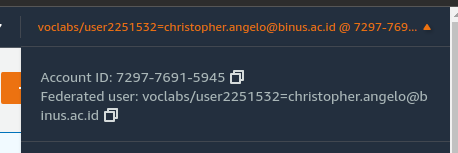
\includegraphics[width=0.5\textwidth]{graphics/section3/AccountId.png}
	\caption{AWS Account ID \& Federated User ID}\label{fig:accid}
\end{figure}

\pagebreak

\subsection*{Cloud Security: Answer 3}

In this lab, I will be working with 4 users under my IAM control panel: `awsstudent', `user-1', `user-2', and `user-3'.

\begin{figure}[H]
	\centering
	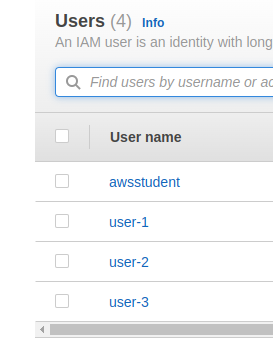
\includegraphics[width=0.25\textwidth]{graphics/section3/IAMUsers.png}
	\caption{AWS IAM Accounts}\label{fig:iamacc}
\end{figure}

\subsection*{Cloud Security: Answer 4}

There are also 3 user groups under my IAM control panel: `EC2-Admin', `EC2-Support' and `S3-Support'.

\begin{figure}[H]
	\centering
	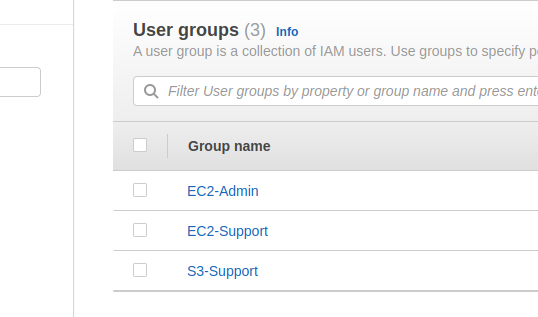
\includegraphics[width=0.475\textwidth]{graphics/section3/IAMUserGroups.png}
	\caption{AWS IAM User Groups}\label{fig:iamusergroup}
\end{figure}

\subsection*{Cloud Security: Answer 5}

In this lab assignment, we are assigning the following users to the following group:

\begin{itemize}
	\item `user-1' to `S3-Support'
	\item `user-2' to `EC2-Support'
	\item `user-3' to `EC2-Admin'
\end{itemize}

\begin{figure}[H]
	\centering
	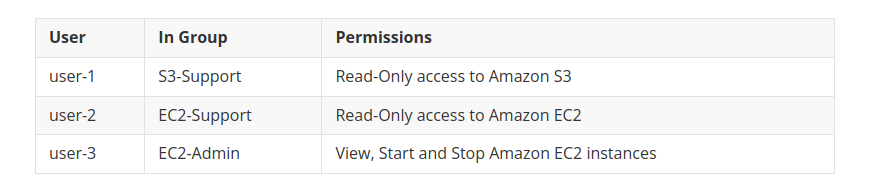
\includegraphics[width=0.75\textwidth]{graphics/section3/IAMUserGroupAssigned.png}
	\caption{Assigned AWS IAM User Groups}\label{fig:iamusergroupassigned}
\end{figure}

\pagebreak

\begin{problem}
\begin{enumerate}
	\setcounter{enumi}{5}
	\item Mention the members (IAM users) included in any User Group in the lab you are working on!
	\item You log in using the IAM user that has been created, include a screenshot of the login result, by showing Regions, User ID
	\item With the IAM user credential already created in the lab, Login using that IAM USER which has credentials to log in to Amazon S3 Buckets. Mention the IAM credential and include a screenshot by including the user id data, Amazon S3 instance!
	\item With the IAM user credential that has been created in the lab, Login using the IAM USER which has credentials to log in to the EC2 server. Mention the IAM credential and include a screenshot by including the user id data, EC2 instance!
\end{enumerate}
\end{problem}

\subsection*{Cloud Security: Answer 6} Duplicate question with question 5

\subsection*{Cloud Security: Answer 7 \& 8}

After logging in with `user-1', the following is the account's User ID and Region. The account is based in `us-east-1' (US East, North Virginia), and their User ID is 265711335029.

\begin{figure}[H]
	\centering
	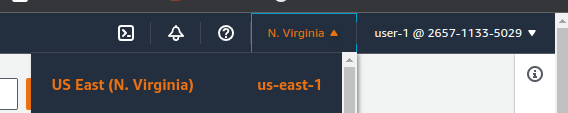
\includegraphics[width=0.75\textwidth]{graphics/section3/IAMUser1AccIdZone.png}
	\caption{IAM Account `user-1' details}\label{fig:iamloginuser1}
\end{figure}

Inside the`user-1' account, there has been a S3 bucket that has been created `samplebucket\-2b323230'

\begin{figure}[H]
	\centering
	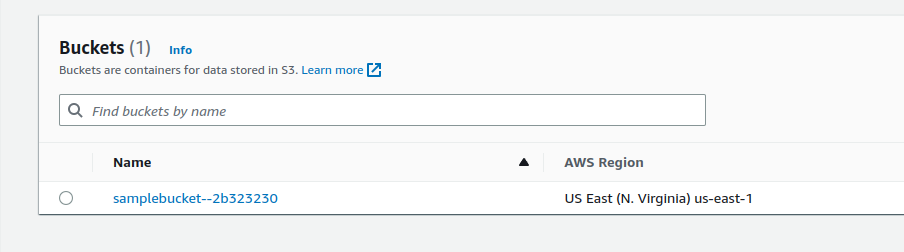
\includegraphics[width=0.9\textwidth]{graphics/section3/IAMUser1S3.png}
	\caption{IAM Account `user-1' S3}\label{fig:iamloginuser1s3}
\end{figure}

\pagebreak

\subsection*{Cloud Security: Answer 9}

After logging in with `user-3', the following is the account's User ID and Region. The account is based in `us-east-1' (US East, North Virginia), and their User ID is 265711335029.

\begin{figure}[H]
	\centering
	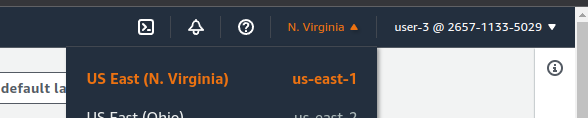
\includegraphics[width=0.8\textwidth]{graphics/section3/IAMUser3AccIdZone.png}
	\caption{IAM Account `user-3' details}\label{fig:iamloginuser3}
\end{figure}

Inside the`user-3' account, there is two t2.micro EC2 instances that is running named `LabHost' and `BastionHost'.

\begin{figure}[H]
	\centering
	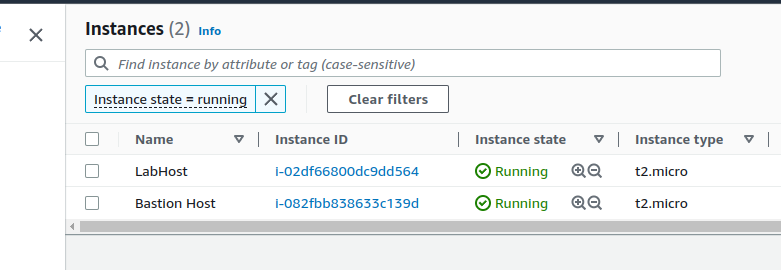
\includegraphics[width=0.8\textwidth]{graphics/section3/IAMUser3EC2.png}
	\caption{IAM Account `user-3' details}\label{fig:iamloginuser3ec2}
\end{figure}

\pagebreak

\section*{Learning Objective 3 and 4 --- VPC \& EC2}

\begin{problem}
Each student is expected to run the AWS Lab on AWS Academy module 5 --- Networking \& Content Delivery --- Lab2 --- Build your VPC and Launch a Web Server, pay attention to the steps in the lab and answer the questions below:

\medskip

\begin{enumerate}
	\item Mention the Region where your Lab is located! include a screenshot!
	\item In that lab, how many Available zones are used? And explain the function of the Available Zone in the lab system!
	\item State the IP address on the system:
	      \begin{enumerate}
		      \item Range IP address for the Lab Regions!
		      \item Public IP Range for Available Zone A
		      \item Public IP Range for Available Zone B
		      \item Private IP Range for Available Zone A
		      \item Public IP Range for Available Zone B
	      \end{enumerate}
\end{enumerate}
\end{problem}

\subsection*{VPC \& EC2: Answer 1}

The region that I am working on is `us-east-1' (US East, North Virginia).

\begin{figure}[H]
	\centering
	\includegraphics[width=0.9\textwidth]{graphics/section4/Zone.png}
	\caption{AWS Region}\label{fig:vpcregion}
\end{figure}

\subsection*{VPC \& EC2: Answer 2}

In this lab, there are 2 available zones in the region that I will be working on: `us-east-1a' and `us-east-1b'. The available zones in this lab are being functioned as resiliency, making sure that the system is still up and running even if one of the available zones is down (higher availability).

\subsection*{VPC \& EC2: Answer 3}

The following are the IP address for the lab system:

\begin{itemize}
	\item Range IP address for the Lab Regions: 10.0.0.0/16
	\item Public IP Range for Available Zone A\@: 10.0.0.0/24
	\item Public IP Range for Available Zone B\@: 10.0.2.0/24
	\item Private IP Range for Available Zone A\@: 10.0.1.0/24
	\item Public IP Range for Available Zone B\@: Duplicate question, if private: 10.0.3.0/24
\end{itemize}

\pagebreak

\begin{problem}
\begin{enumerate}
	\setcounter{enumi}{3}
	\item In the lab the term AMI (Amazon Machine Image) is known, explain the function of the AMI\@!
	\item Mention the applications installed on the EC2 web servers!
	\item Mention the Public DNS created on the server!
\end{enumerate}
\end{problem}

\subsection*{VPC \& EC2: Answer 4}

AMI (Amazon Machine Image) is a template that contains a software configuration: operating system, application server, and applications (think of an \@.iso file). The AMI is used to launch an EC2 instance. A custom AMI is internally stored in Amazon S3, and can be copied across regions for deployment in other zones.

\subsection*{VPC \& EC2: Answer 5}

When deploying the EC2 instance, there is an install script that is being run to install Apache Web Server and PHP (more formally installed `httpd', `mysql' and `php' through `yum' package manager)

\subsection*{VPC \& EC2: Answer 6}

The public DNS for the EC2 instance is `ec2-3-84-206-67.compute-1.amazonaws.com'

% \printbibliography[]{}

\end{document}
